\documentclass[10pt]{article}
\usepackage{amsmath,amsfonts,times}
\usepackage{graphicx,color,tikz,pgfplots}
\usepackage[paperwidth=13cm,paperheight=6.5cm,lmargin=0in,rmargin=0in,tmargin=0.in,bmargin=0.in]{geometry}
\usepackage{bm}
\usetikzlibrary{arrows,shadings,shapes.arrows,decorations.pathreplacing,calc, positioning}
\usepgfplotslibrary{fillbetween}

\pgfplotsset{compat=1.15,
  myStyle/.style={
    width=7cm,
    height=7cm,
    xmin=0,
    xmax=1,
    ymin=0,
    ymax=1,
    axis line style=ultra thick, 
    colormap/bluered,
    colorbar,
    ticks=none,
    colorbar style={
      title=Weights,
      at={(1.1,0)},anchor=south west }
  },
}


\begin{document}
\centering
\begin{tikzpicture}
  \node[alias=armadillo] at (0,0) {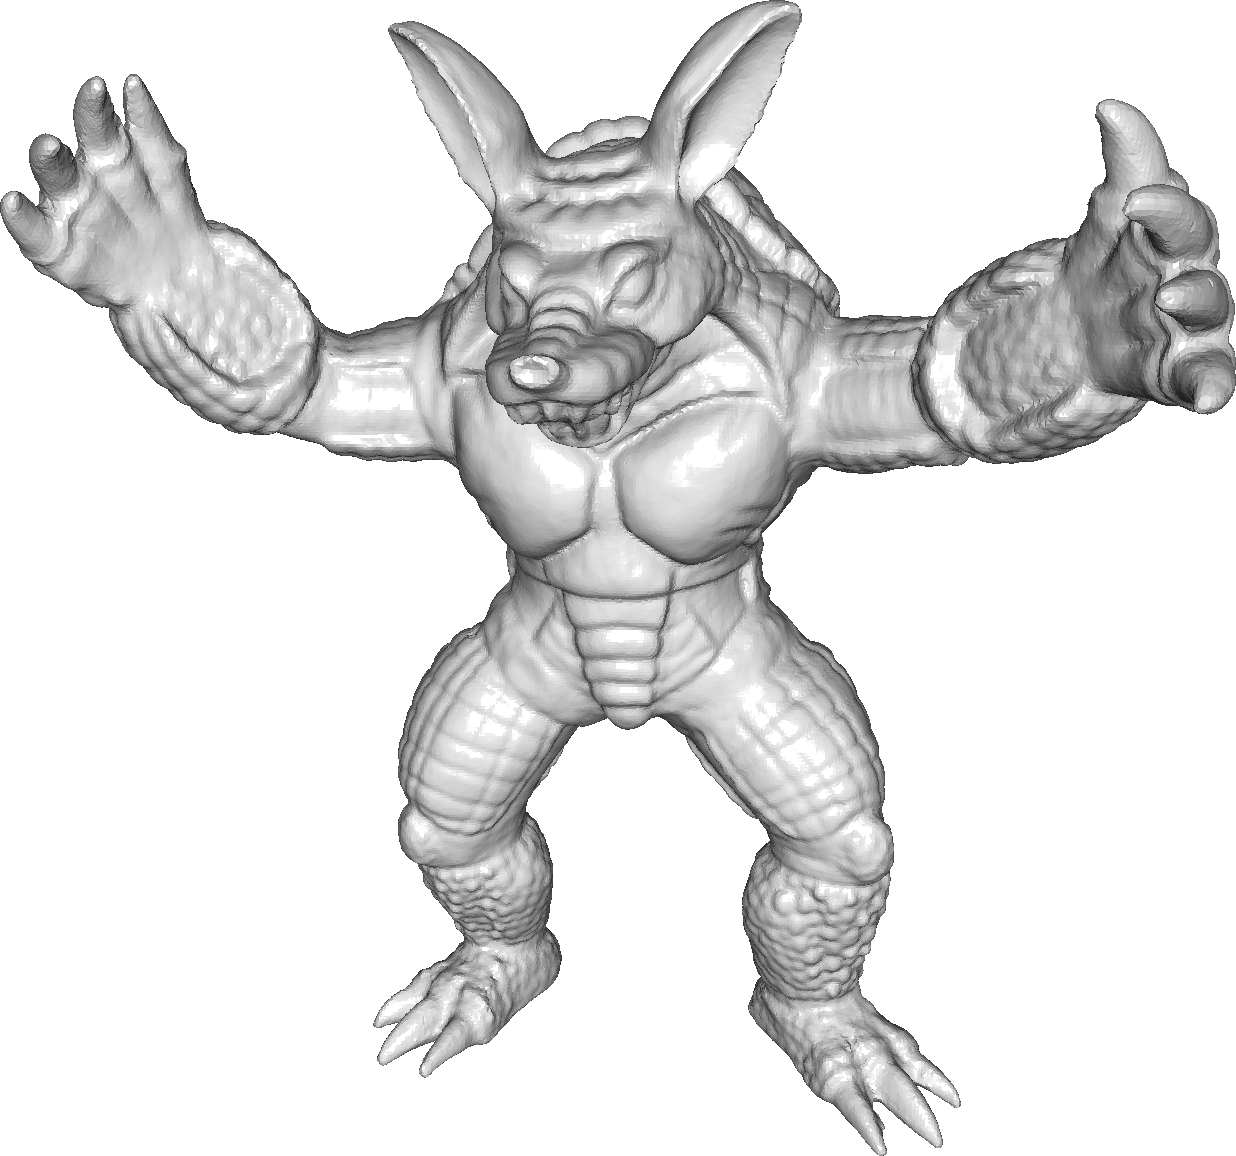
\includegraphics[height=3cm]{armadillo}};
  \node[alias=hind, right=0cm of armadillo] {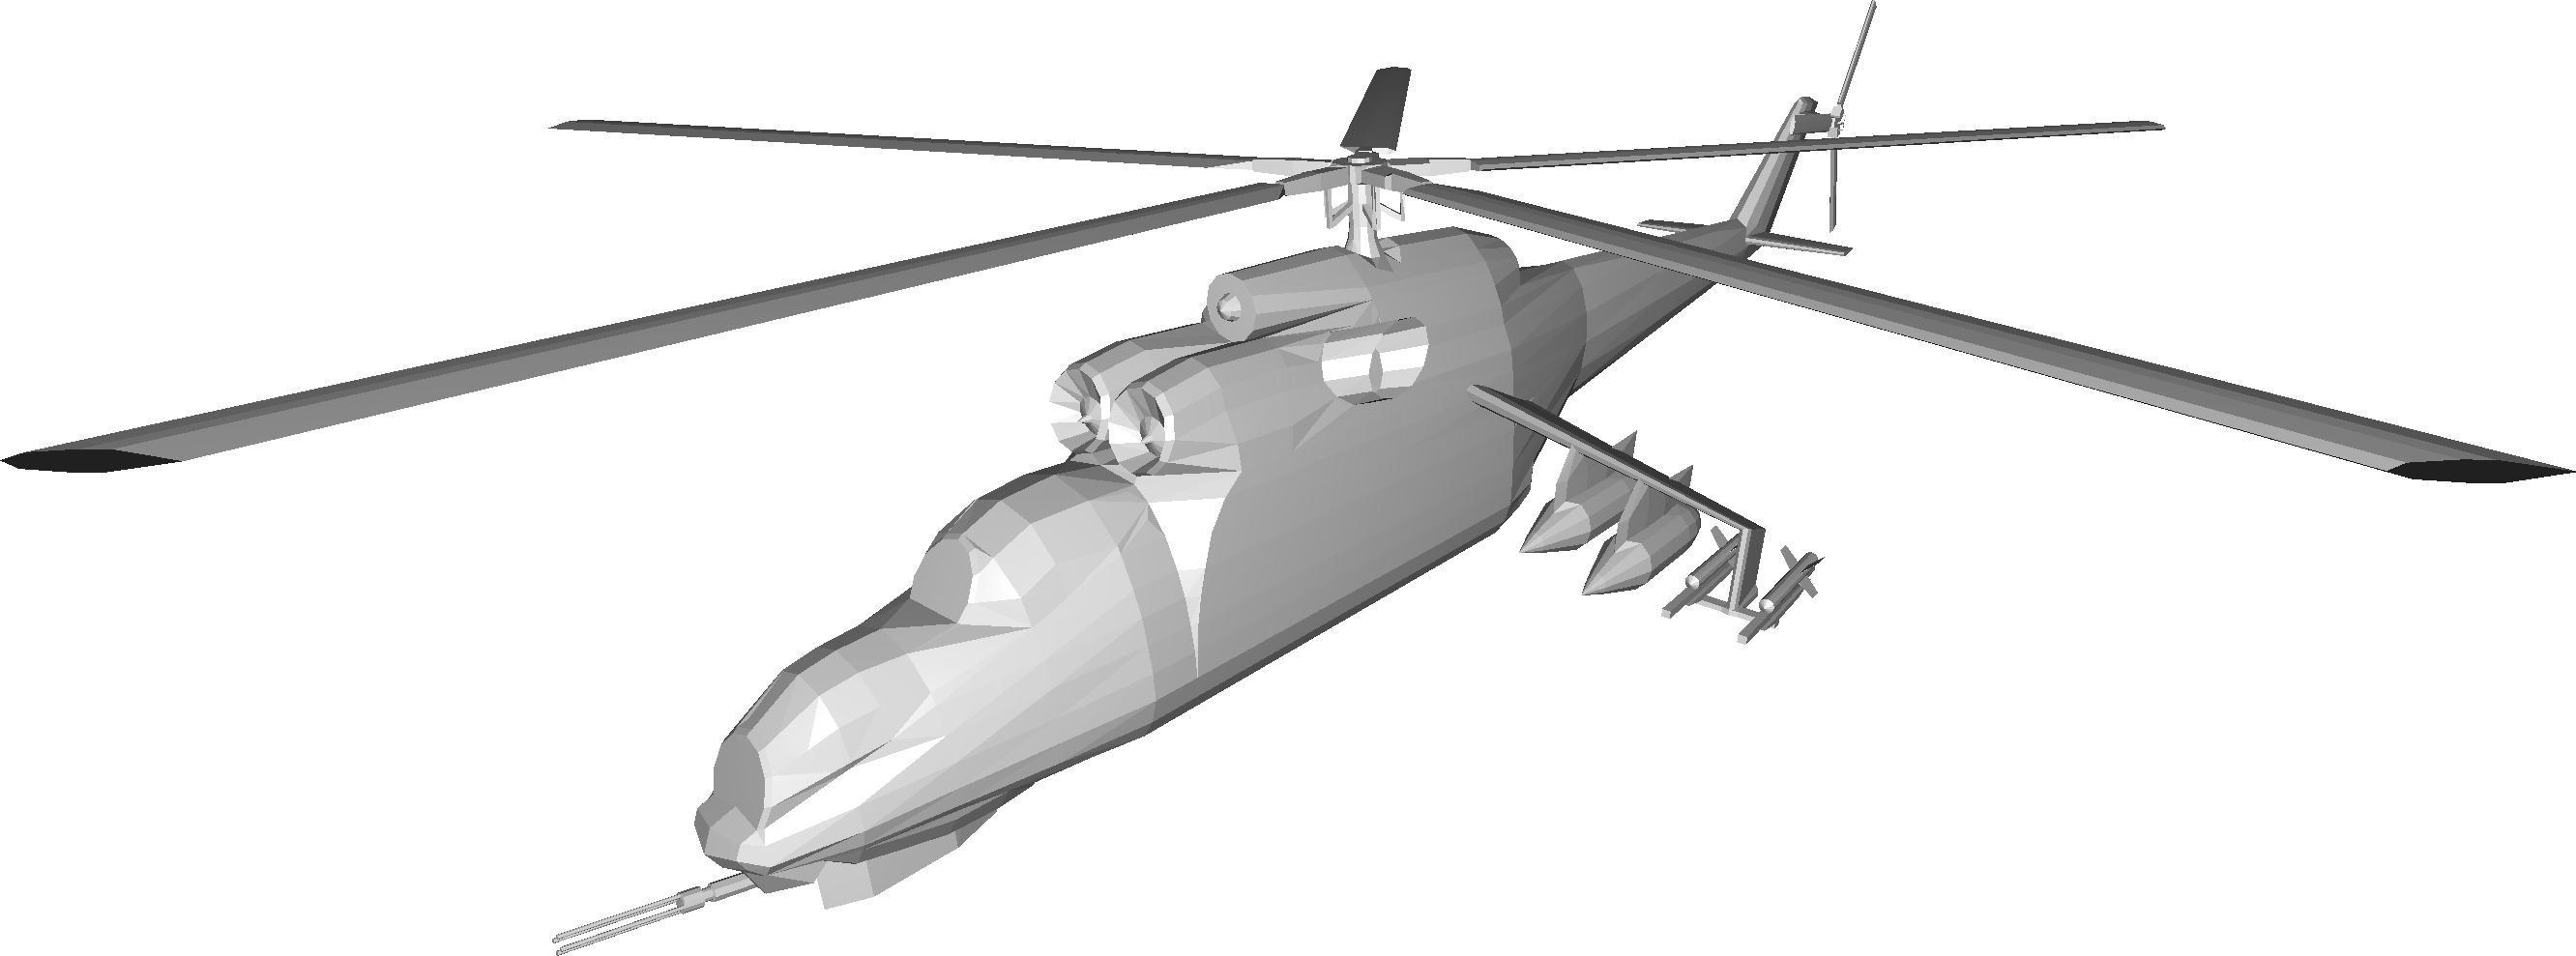
\includegraphics[height=3cm]{hind}};
  \node[alias=orion, below=0cm of armadillo]  {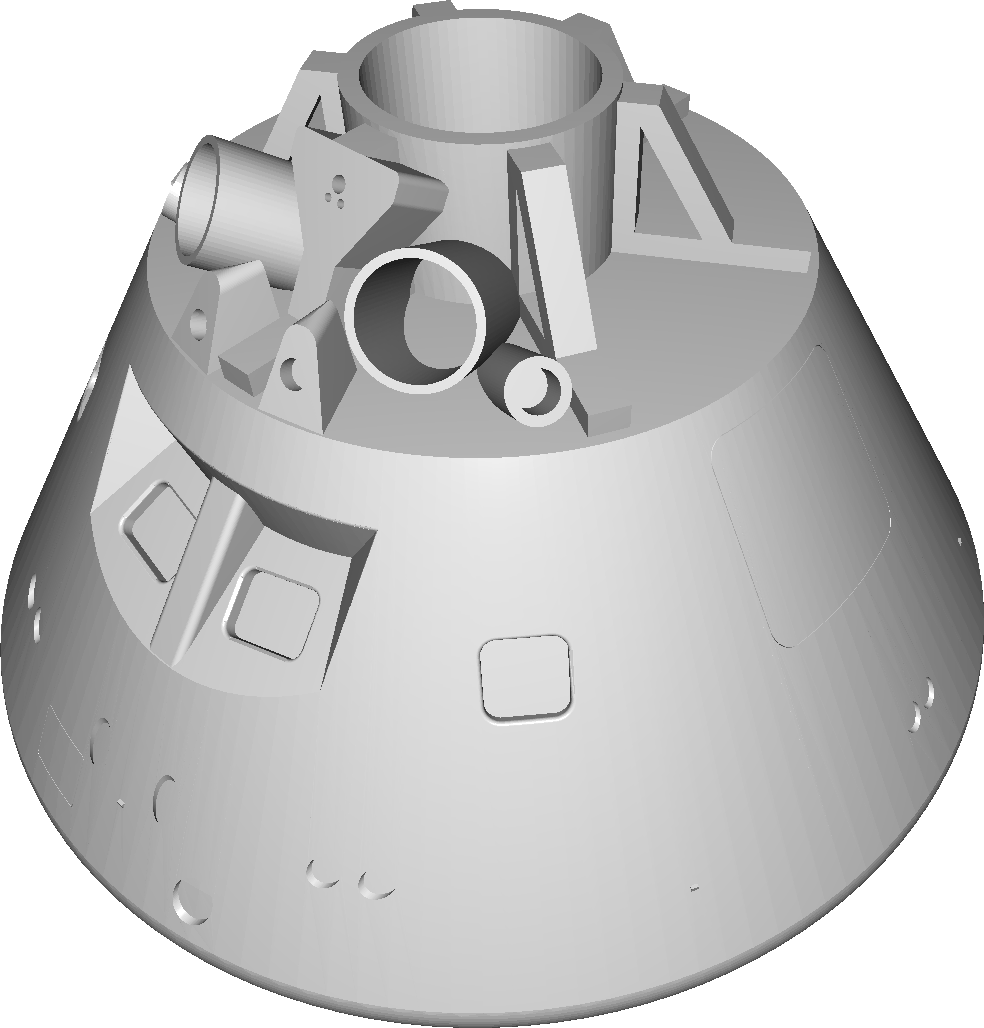
\includegraphics[height=3cm]{orion}};
  \node[alias=porsche, below=0cm of hind]  {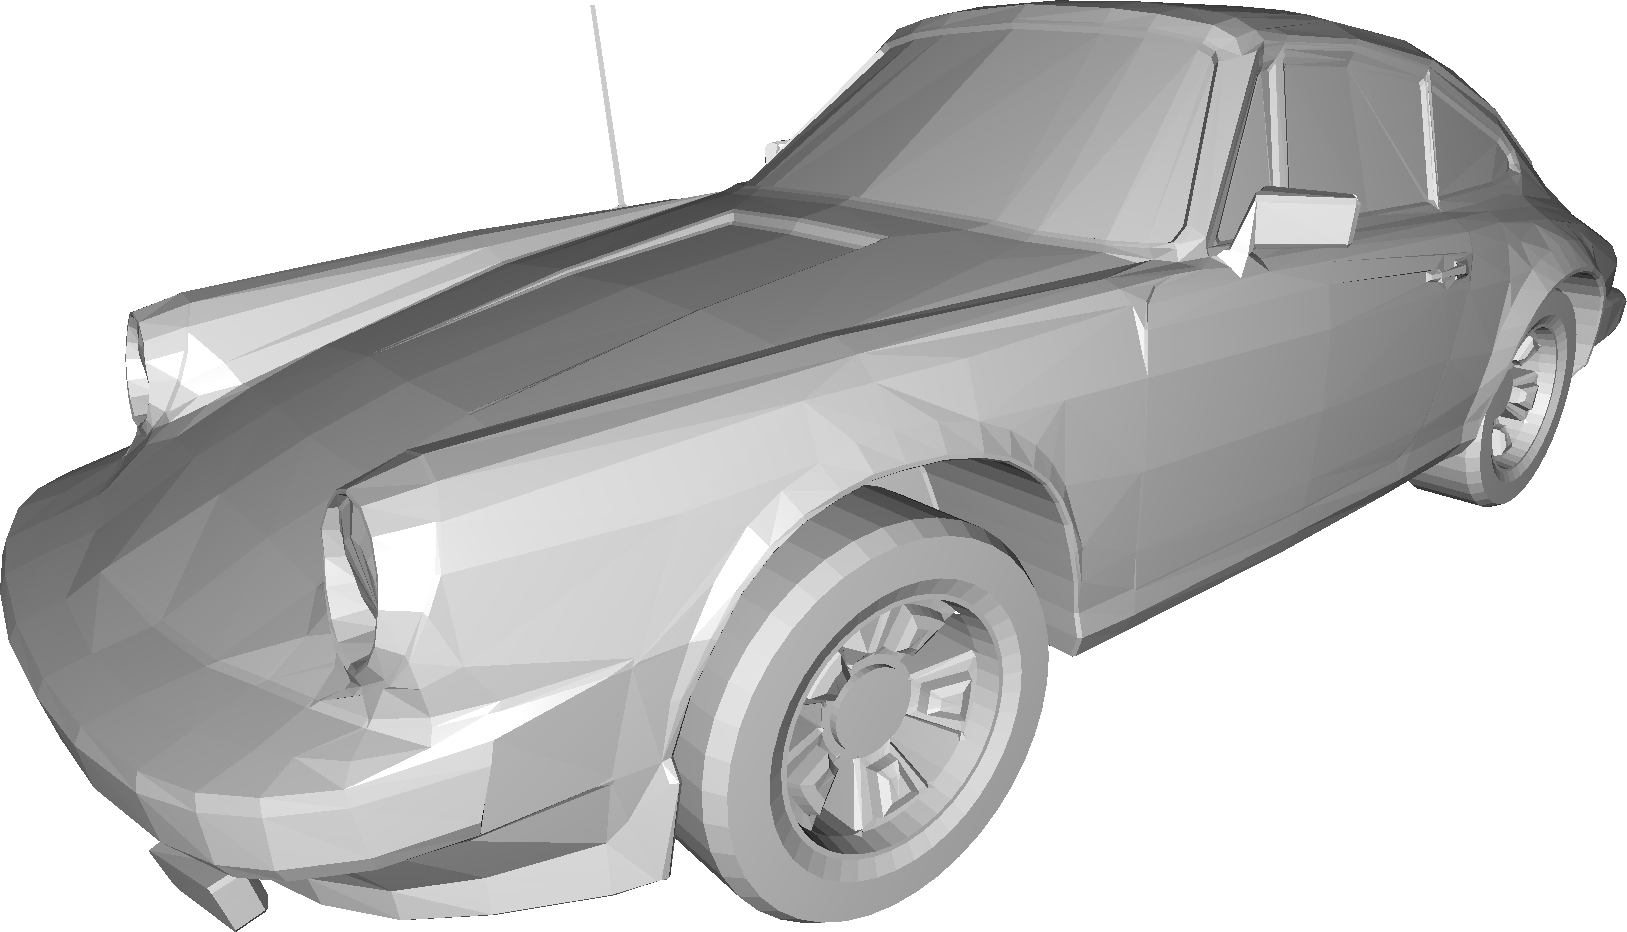
\includegraphics[height=3cm]{porsche}};

\end{tikzpicture}

\end{document} 
